\begin{center}\large\textbf{Readings: Chapter 6 (for 6.3-6.5 read if interested)}\\
\normalsize \end{center}
\large ~\hrulefill
~\\

Our problems so far have dealt with inference for the mean of only \textbf{1 population} of interest.  In real life this will not usually be the case.  We will start with looking at inference regarding the means of \textbf{2 populations} and then in later chapters look at what to do with an arbitrary number of populations.\\~\\

Motivating Example:\\
Jocko's garage seems to be giving out really high estimates for insurance claims.  To investigate insurance fraud, insurance adjusters take 10 damaged cars and take each one to both Jocko's and a repair shop they trust, Jami's repair shop.  Then then get the estimates from the repair shop (in the end, 2 for each car).  Data are provided below: 
\begin{center}
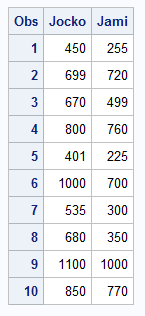
\includegraphics[scale=0.6]{autodata}
\end{center}
Here we have two populations: all estimates from Jocko's and all estimates from Jami's repair shop.\\~\\
Therefore, we have 2 random variables: \\
$Y_i$= estimate for the $i^{th}$ randomly selected car at Jocko's\\
$X_i$= estimate for the $i^{th}$ randomly selected car at Jami's\\~\\

We now have two sample sizes: \\
$n_1$ (or $n_Y$) = number sampled at Jocko's\\ 
$n_2$ (or $n_X$)= number sampled at Jami's.\\
(Here they are equal, but generally for a two sample problem, they need not be.)\\~\\

We now have two sample mean \textbf{random variables}:\\
$\bar{Y}$= mean estimate for a randomly selected sample of 10 cars at Jocko's\\
$\bar{X}$= mean estimate for a randomly selected sample of 10 cars at Jami's\\~\\

We also have 2 sets of summary statistics (1 for each sample):
\begin{center}
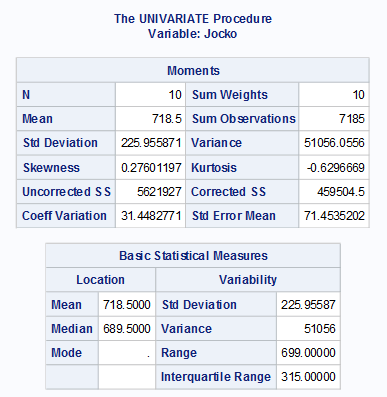
\includegraphics[scale=0.8]{summarycars1}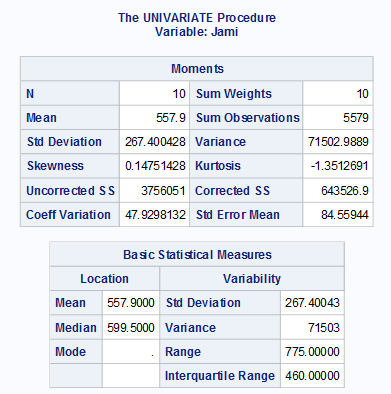
\includegraphics[scale=0.8]{summarycars2}
\end{center}
~\\
Two parameters of interest:\\
$\mu_Y$ (or $\mu_{1}$) = (true) mean of all estimates at Jocko's\\
$\mu_X$ (or $\mu_{2}$) = (true) mean of all estimates at Jami's repair shop.\\~\\
Goal:  Investigate $\mu_{D}=\mu_{diff}=\mu_1-\mu_2=\mu_Y-\mu_X$\\~\\

\newpage

What are possible methods of inference for $\mu_{diff}=\mu_1-\mu_2$?
\begin{center}
\begin{tabular}{c|c|c}
Distribution & Two Samples are Independent & Two Samples are `Paired'\vspace{5pt}\\
$\bar{Y}-\bar{X}\sim Normal$ &  6.2 - Two-sample t-test & 6.4 Paired-t-test\\\vspace{5pt}
$\bar{Y}-\bar{X}\sim Not~Normal$ & 6.3 - Wilcoxon Rank Sum Test & 6.5 - Wilcoxon Signed Rank Test
\end{tabular}
\end{center}
~\\~\\
\Large 6.4 - Inference for Paired Data (Matched Pairs t or Paired t)\normalsize\\~\\

What is paired data?\\
Each `unit' receives two treatments. The units could be: 
\begin{enumerate}
\item A single subject (each subject gets both treatments) 
\item	Two subjects that have been \textbf{matched} together (one receives treatment A and the other receives treatment B) 
\end{enumerate}

Ex: Auto example - We have paired data because\\~\\~\\~\\~\\~\\~\\

How to make inference here?  Hypothesis test = paired t-test:\\
Parameter:\\~\\~\\~\\
Null hypothesis:\\~\\~\\~\\~\\
Alternative Hypothesis:\\~\\~\\~\\~\\~\\~\\~\\~\\~\\
Test Statistic:

\newpage

RR/p-value:\\~\\~\\~\\~\\~\\~\\~\\~\\~\\~\\~\\~\\~\\~\\~\\
Conclusions same as for all HT.  Note that this test is \textbf{equivalent to the one-sample t-test on the differences between the paired data.}\\~\\~\\

Similarly we can create a confidence interval using the test statistic above:
\\~\\~\\~\\~\\~\\~\\~\\~\\~\\~\\~\\~\\~\\~\\~\\~\\~\\~\\~\\~\\~\\~\\~\\~\\~\\~\\
Note:  We do not need to know each variable's sample mean and standard deviation, \textbf{only the mean and standard deviation of the differences!}.
\newpage

Both the HT and the CI can be done very easily in SAS:

\begin{verbatim}
data autodata;
input Jocko Jami;
datalines;
450 255
699 720
670 499
800 760
401 225
1000 700
535 300
680 350
1100 1000
850 770
;

proc ttest data=autodata; 
     paired Jocko*Jami;
run;

/* About this code:
The PAIRED VAR1*VAR2 statement requests the paired t-test. 
SAS calculates the differences as VAR1-VAR2. 
*/
\end{verbatim}

\begin{center}
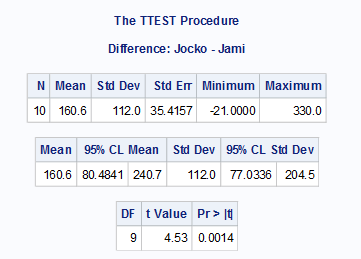
\includegraphics[scale=0.8]{autopaired1}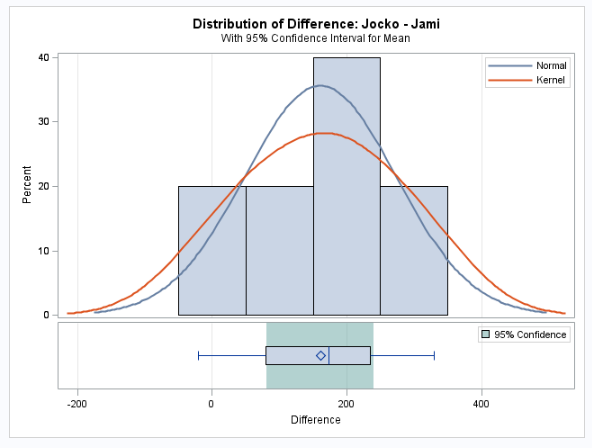
\includegraphics[scale=0.6]{autopaired2}\\
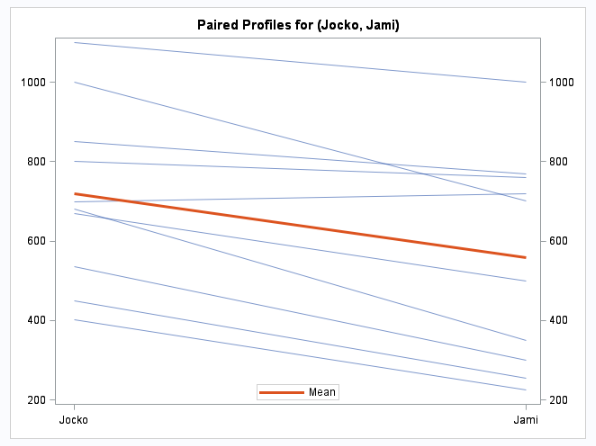
\includegraphics[scale=0.5]{autopaired3}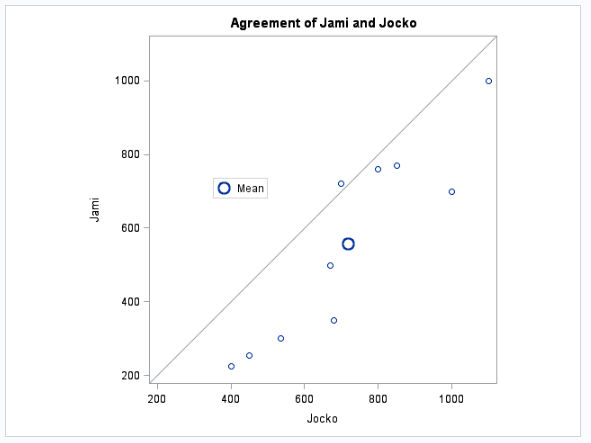
\includegraphics[scale=0.6]{autopaired4}\\~\\~\\~\\~\\
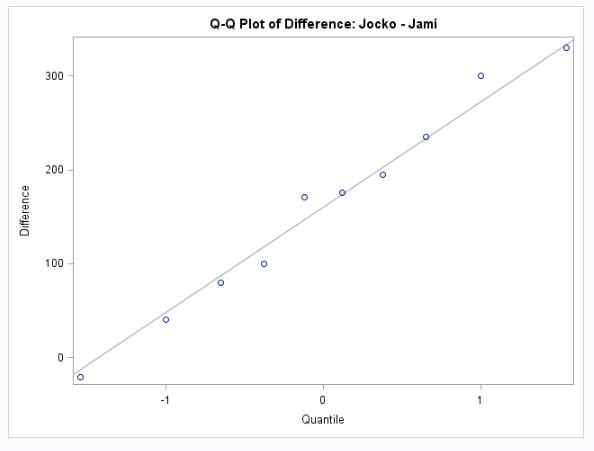
\includegraphics[scale=0.6]{autopaired5}
\end{center}

\newpage

One of the two scenarios below has paired data where looking at paired differences makes sense and on scenario has a case where that does not make any sense (even though paired differences for each are given).  Identify which of the two scenarios below has paired data - for the example with paired data find a 95\% confidence interval (state assumptions needed on the data, how you would inspect the assumption, and interpret the interval):  Some values - $P(T_9>1.83)=0.05~~~P(T_9>2.26)=0.025~~~P(T_{22}>1.72)=0.05~~~P(T_{22}>2.07)=0.025$
\begin{enumerate}
\item A nutrition expert is examining a weight loss program to evaluate its effectiveness (i.e., if participants lose weight on the program). Ten subjects are randomly selected for the investigation. Each subject’s initial weight is recorded, they follow the program for 6 weeks, and they are again weighed. Is the program effective?\\
The data are given below:
\begin{multicols}{2}
\begin{tabular}{c|cc}
Subject	&Initial Weight	&Final Weight\\\hline
1&	180&	165\\
2&	142&	138\\
3&	126&	128\\
4&	138&	136\\
5&	175&	170\\
6&	205&	197\\
7&	116&	115\\
8&	142&	128\\
9&	157&	144\\
10&	136&	130\\
\end{tabular}
\columnbreak
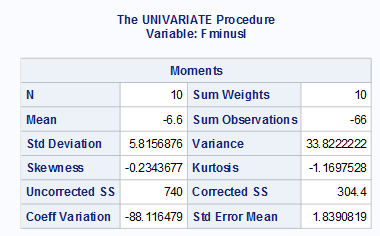
\includegraphics[scale=0.8]{weightdiff}
\end{multicols}
~\\~\\~\\~\\~\\
\item A manufacturer of cat food wants to assure that the packages being produced at the Tennessee plant have the same average weight as the packages being produced at the Wisconsin plant. Samples of 23 packages each were collected from Tennessee plant and Wisconsin plant respectively. The package weights (in ounces) are given below:
\end{enumerate}
\begin{multicols}{2}
\begin{tabular}{c|cc}
Sample & Tennessee & Wisconsin\\\hline
1 & 4.67 & 4.74\\
2 & 4.65 & 4.65\\
3 & 4.68 & 4.60\\
4 & 4.59 & 4.62\\
\vdots & \vdots & \vdots\\
23& 4.66 & 4.62
\end{tabular}
\columnbreak
~\\~\\
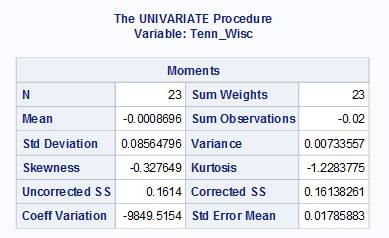
\includegraphics[scale=0.75]{catfooddiff}
\end{multicols}

\newpage

Output from SAS to conduct the paired t-test on the weight example.
\begin{multicols}{2}
*Conduct paired t-test;\\
proc ttest data=weight;\\
paired Final*Initial;\\
run; 
\columnbreak
\begin{center}
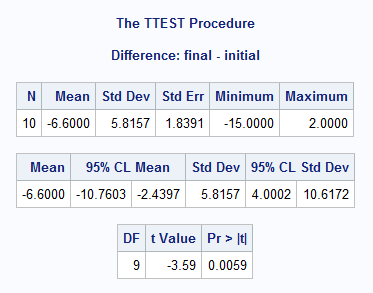
\includegraphics[scale=0.7]{weightoutput}
\end{center}
\end{multicols}
~\\
\Large 6.2 - Inference for Two Independent Samples (Two-Sample t)\normalsize\\~\\

For the second example on the previous page, we did not have paired data, but rather two samples, one from the Tennessee population and one from the Wisconsin population. 
\begin{center}
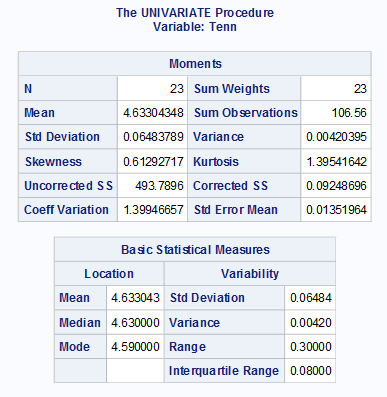
\includegraphics[scale=0.70]{catTenn}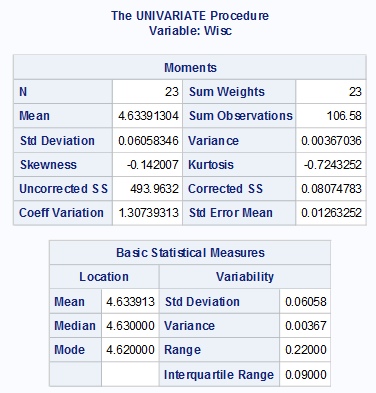
\includegraphics[scale=0.70]{catWisc}\\
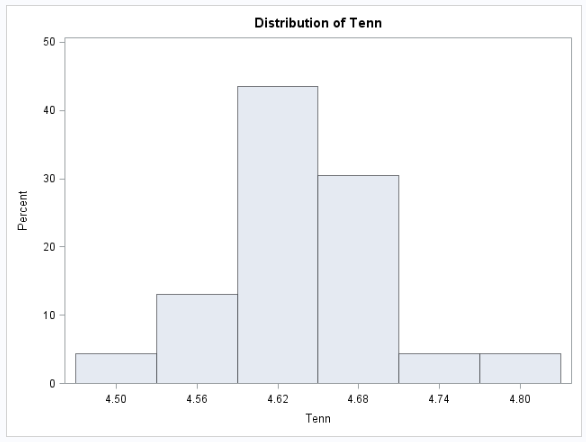
\includegraphics[scale=0.35]{catTenn2}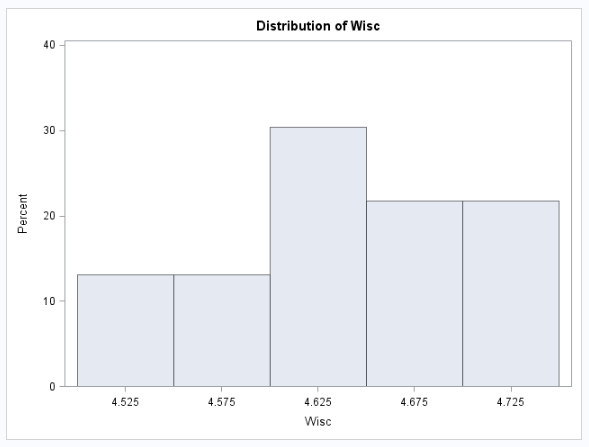
\includegraphics[scale=0.35]{catWisc2}
\end{center}
Define:\\
$Y_i$ = the weight for the $i^{th}$ randomly selected package from the Tennessee plant\\
$X_i$ = the weight for the $i^{th}$ randomly selected package from the Wisconsin plant\\~\\
$\mu_{1} =$ the mean weights for Tennessee plants\\
$\mu_{2} = $ the mean weights for Wisconsin plants \\~\\~\\~\\
%mu_d
Question of interest (Claim):\\~\\~\\~\\~\\~\\~\\~\\

What could we do to make inference here?\\~\\
An `unbiased' estimate of $\mu_d$ is \\~\\~\\~\\~\\~\\~\\~\\~\\~\\~\\~\\ %So our inference should revolve around this quantity
What is the variance of this quantity?\\~\\
Let's define the \underbar{~~~~~~~~~~~~~~~~~~~~~~~~~~~~~~~~} between two random variables.  $Cov(X,Y)$ is a measure the how\\~\\ the random variables \underbar{~~~~~~~~~~~~~~~~~~~~~~~~~~~~~~~~~~~~~~~~~~~~~~~~~~~~~~~~~~~~~~~~~~~~~~}\\~\\
Mathematically: 
$$Cov(X,Y)=E(XY)-E(X)E(Y) \mbox{ - Similar to }Var(X)=E(X^2)-\left(E(X)\right)^2 = E(XX)-E(X)E(X)$$
Generally, for the random variable $aX+bY$ we have
$$Var(aX+bY) = a^2Var(X)+b^2Var(Y)+2abCov(X,Y)$$~\\
Since covariance is a measure of how the RV's vary together.  If $X$ is independent of $Y$ that means\\~\\~\\~\\
~~~~~~~~~~~~~~~This implies that if $X$ is independent of $Y$ then $Cov(X,Y)=0$.
\newpage

Now back to our quantity $\bar{D}$, what is the variance of this quantity?\\~\\~\\~\\~\\~\\~\\~\\~\\~\\
Knowing the mean and variance of this quantity is useful, but to use it for inference we must know the\\~\\~\\~\\~\\

Theorem:  If $Y_i\sim^{iid}N(\mu_1,\sigma^2)$ and $X_i\sim^{iid}N(\mu_2,\sigma^2)$ (both parent populations are normal, same variance) where all $Y$ are \textbf{independent} of all $X$ (independent samples) then\\~\\~\\~\\~\\~\\~\\~\\~\\
We can estimate the common variance by\\~\\~\\~\\~\\~\\~\\~\\~\\~\\~\\~\\~\\
Thus, the \textbf{test statistic} we can use for our HT and CI are
%Called pooled-t test/CI

\newpage

ex:  Back to the catfood example.  Let us assume that $Y_i\sim^{iid}N(\mu_1,\sigma^2)$ and $X_i\sim^{iid}N(\mu_2,\sigma^2)$ where $Y's$ and $X's$ are independent (that is, our parent populations are independent normals with equal variance assumed).  Let's conduct a hypothesis test at the 0.01 level to determine if the mean weights differ.  Would a 99\% CI for $\mu_{diff}$ contain 0?  Why/why not?

\newpage
\begin{multicols}{2}
Analysis of cat food data using SAS\\~\\
proc ttest data=catfood2;\\
*Specify that location is categorical;\\
class location;\\
*variable that we want to test on;\\
var weight;\\
run;\\
\columnbreak
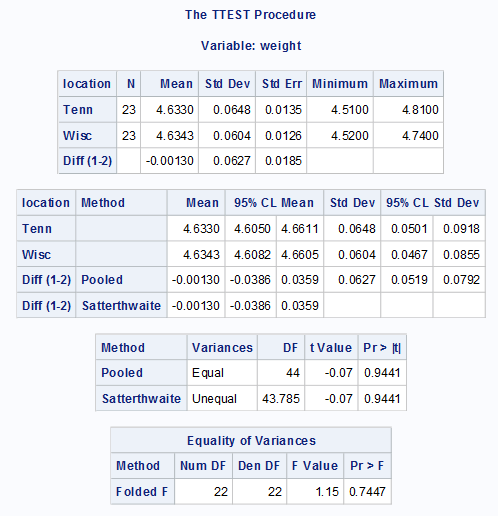
\includegraphics[scale=0.75]{catfoodttest}
\end{multicols}
\begin{center}
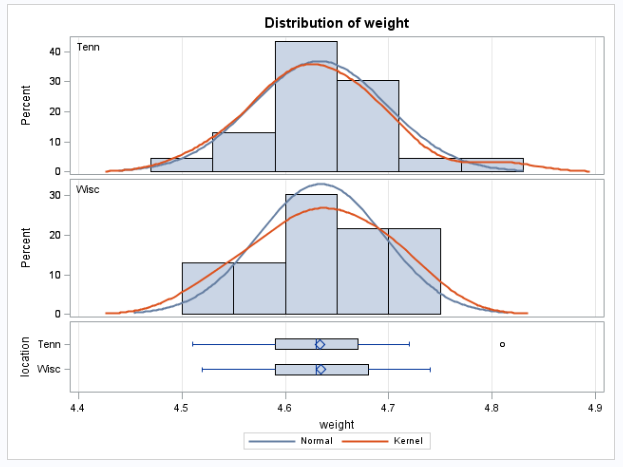
\includegraphics[scale=0.55	]{catfoodplot1}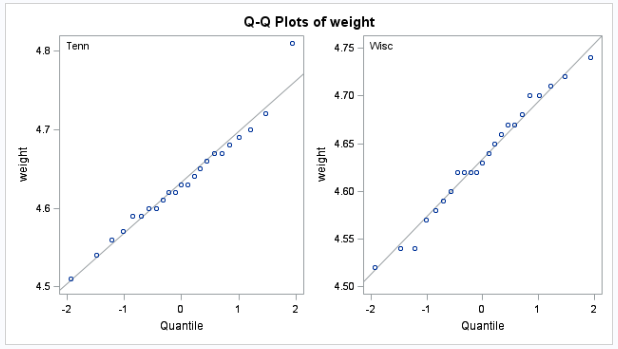
\includegraphics[scale=0.55]{catfoodplot2}
\end{center}

\newpage

The equal variance assumption seemed reasonable above.  What can we do when it is \textbf{not} reasonable?\\~\\

Theorem:  If $Y_i\sim^{iid}N(\mu_1,\sigma^2_1)$ and $X_i\sim^{iid}N(\mu_2,\sigma^2_2)$ (both parent populations are normal, different variance) where all $Y$ are \textbf{independent} of all $X$ (independent samples) then\\~\\~\\~\\~\\~\\~\\~\\~\\

Therefore, $\bar{D}=\bar{Y}-\bar{X}$ still is a good statistic to base our inference on.\\~\\~\\
Suppose we estimate our standard error using the sample variances:\\~\\~\\~\\~\\~\\

We can create the test statistic\\~\\~\\~\\~\\~\\
Issue:  What are the degrees of freedom for our test statistic??\\~\\~\\~\\~\\~\\~\\

\textbf{Satterthwaite's approximation to degrees of freedom}\\
To approximate the $df$ associated with a $t$ statistic based on a standard error of the form
$$ SE = \sqrt{c_1 S^2_1 + c_2 S^2_2 + \cdots + c_k S^2_k}$$
(a linear combination of sample variances), use the \textbf{Satterthwaite approximation:}
$$ \widehat{df} = \frac{(c_1 S^2_1 + c_2 S^2_2 + \cdots + c_k S^2_k)^2}{(c_1 S^2_1)^2/df_1 + (c_2 S^2_2)^2/df_2 + \cdots + (c_k S^2_k)^2/df_k}$$
Always round down!
%Called the 2 sample t-test
\newpage

Example: Consider an experiment involving the comparison of the mean heart rate following 30 minutes of aerobic exercise among females aged 20 to 24 years (Y variable, group 1) as compared to females aged 30-34 years (X variable, group 2). For this experiment, heart rates are recorded on each participant following 30 minutes of intense aerobic exercise.  The sample data and some statistics (not all will be needed) are given below:\\
$n_1 = 15$, $\bar{y}$=150.22, $s^2_1$ = 160\\
$n_2 = 10$, $\bar{x}$ = 141.10, $s^2_2$ = 100\\
$$\widehat{SE}\left(\bar{Y}-\bar{X}\right)=\sqrt{\frac{(n_1-1)s_1^2+(n_2-1)s_2^2}{n_1+n_2-2}\left(\frac{1}{n_1}+\frac{1}{n_2}\right)}=\sqrt{\frac{(15-1)160+(10-1)100}{15+10-2}\left(1/15+1/10\right)}=4.768$$
$$\widehat{SE}\left(\bar{Y}-\bar{X}\right)=\sqrt{\frac{s_1^2}{n_1}+\frac{s_2^2}{n_2}} = \sqrt{\frac{160}{15}+\frac{100}{10}} = 4.55$$
$$\widehat{df} = \frac{\left(\frac{s_1^2}{n_1}+\frac{s_2^2}{n_2}\right)^2}{\left(\frac{s_1^2}{n_1}\right)^2/(n_1-1)+\left(\frac{s_2^2}{n_2}\right)^2/(n_2-1)}=\frac{\left(\frac{160}{15}+\frac{100}{10}\right)^2}{\left(\frac{160}{15}\right)^2/(15-1)+\left(\frac{100}{10}\right)^2/(10-1)}=22.20$$
$$P(T_{23}>2.50)=0.01~~~P(T_{23}>2.81)=0.005~~~P(T_{22}>2.51)=0.01~~~~P(T_{22}>2.82)=0.005$$
Conduct a hypothesis test at the $\alpha=0.01$ level assuming the variances of the two population are not equal.  Be sure to show all steps (use RR, state the assumptions that must be made and how you would check that assumption). Also, create a 99\% confidence interval for the difference in means.

\newpage

\begin{multicols}{2}
Analysis of heart rate data using SAS\\~\\
proc ttest data=heartrate;\\
*denote group as a categorical variable;\\
class group;\\
var rate;\\
run;\\
\columnbreak
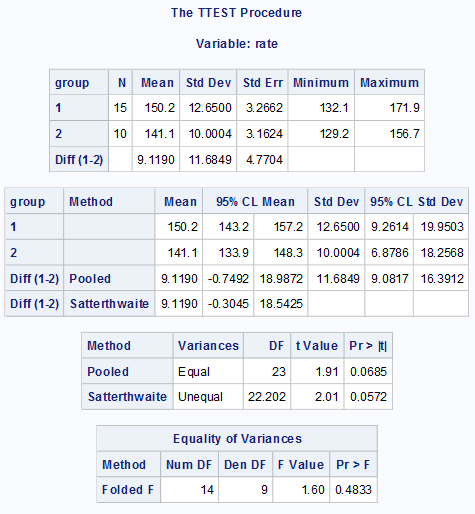
\includegraphics[scale=0.75]{heartratettest}
\end{multicols}
\begin{center}
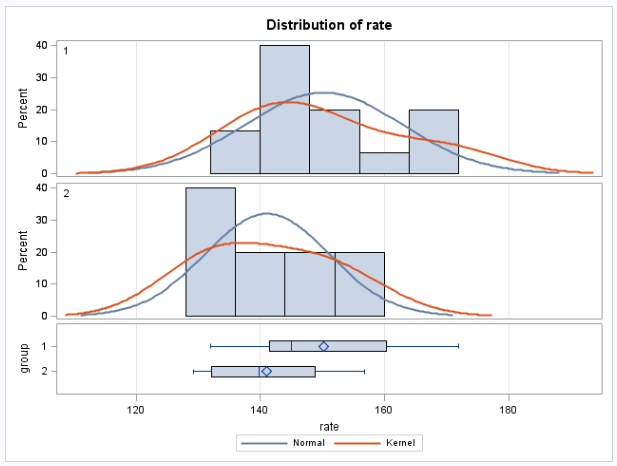
\includegraphics[scale=0.55	]{heartrateplot1}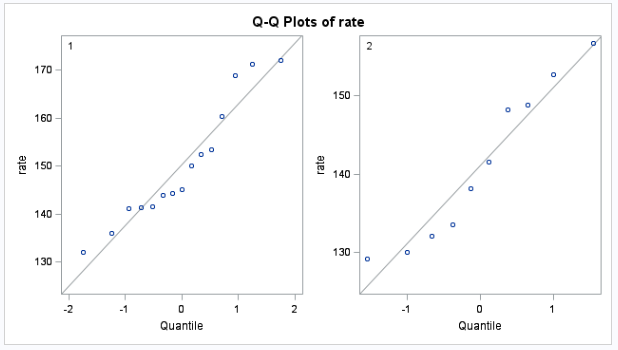
\includegraphics[scale=0.55]{heartrateplot2}
\end{center}

\newpage

\large Recap of possible inferences for the difference of means based on the normal distribution:\normalsize\\~\\
\textbf{Paired Data:}  Assume \textbf{differences} are a RS and normally distributed\\
100(1-$\alpha$)\% CI for $\mu_d$ is
$$\overline{D}\pm t_{\alpha/2,n-1}S_D/\sqrt{n} = \bar{Y}-\bar{X}\pm t_{\alpha/2,n-1}S_{\bar{Y}-\bar{X}}/\sqrt{n}$$
HT: for $H_0:\mu_d=\Delta_0~~vs~~H_a: \mu_d>\Delta_0~~or~~\mu_d<\Delta_0~~or~~\mu_d\neq\Delta_0$
$$\mbox{Test Statistic: } T=\frac{\bar{Y}-\bar{X}-\Delta_0}{S_d/\sqrt{n}}$$
$$RR: \left\{t_{obs}:t_{obs}>t_{\alpha,n-1}\right\}~~or~~\left\{t_{obs}:t_{obs}<-t_{\alpha,n-1}\right\}~~or~~\left\{t_{obs}:|t_{obs}|>t_{\alpha/2,n-1}\right\}$$
$$P-value: P(T_{n-1}>t_{obs})~~or~~P(T_{n-1}<t_{obs})~~or~~2*P(T_{n-1}>|t_{obs}|)$$
~\\
\textbf{Independent Samples:} Assume populations are independent RS's with each population having a normal distribution\\
\textbf{Equal Variance} (Pooled Variance):\\
100(1-$\alpha$)\% CI for $\mu_d$ is
$$\bar{Y}-\bar{X}\pm t_{\alpha/2,n_1+n_2-2}\sqrt{\frac{(n_1-1)s_1^2+(n_2-1)s_2^2}{n_1+n_2-2}\left(\frac{1}{n_1}+\frac{1}{n_2}\right)}$$
HT: for $H_0:\mu_d=\Delta_0~~vs~~H_a: \mu_d>\Delta_0~~or~~\mu_d<\Delta_0~~or~~\mu_d\neq\Delta_0$
$$\mbox{Test Statistic: } T=\frac{\bar{Y}-\bar{X}-\Delta_0}{\sqrt{\frac{(n_1-1)s_1^2+(n_2-1)s_2^2}{n_1+n_2-2}\left(\frac{1}{n_1}+\frac{1}{n_2}\right)}}$$
$$RR: \left\{t_{obs}:t_{obs}>t_{\alpha,n_1+n_2-2}\right\}~~or~~\left\{t_{obs}:t_{obs}<-t_{\alpha,n_1+n_2-2}\right\}~~or~~\left\{t_{obs}:|t_{obs}|>t_{\alpha/2,n_1+n_2-2}\right\}$$
$$P-value: P(T_{n_1+n_2-2}>t_{obs})~~or~~P(T_{n_1+n_2-2}<t_{obs})~~or~~2*P(T_{n_1+n_2-2}>|t_{obs}|)$$
~\\
\textbf{Unequal Variance:}\\
100(1-$\alpha$)\% CI for $\mu_d$ is
$$\bar{Y}-\bar{X}\pm t_{\alpha/2,\widehat{df}}\sqrt{\frac{s_1^2}{n_1}+\frac{s_2^2}{n_2}}$$
HT: for $H_0:\mu_d=\Delta_0~~vs~~H_a: \mu_d>\Delta_0~~or~~\mu_d<\Delta_0~~or~~\mu_d\neq\Delta_0$
$$\mbox{Test Statistic: } T=\frac{\bar{Y}-\bar{X}-\Delta_0}{\sqrt{\frac{s_1^2}{n_1}+\frac{s_2^2}{n_2}}}$$
$$RR: \left\{t_{obs}:t_{obs}>t_{\alpha,\widehat{df}}\right\}~~or~~\left\{t_{obs}:t_{obs}<-t_{\alpha,\widehat{df}}\right\}~~or~~\left\{t_{obs}:|t_{obs}|>t_{\alpha/2,\widehat{df}}\right\}$$
$$P-value: P(T_{\widehat{df}}>t_{obs})~~or~~P(T_{\widehat{df}}<t_{obs})~~or~~2*P(T_{\widehat{df}}>|t_{obs}|)$$
$$\widehat{df}=\frac{\left(\frac{s_1^2}{n_1}+\frac{s_2^2}{n_2}\right)^2}{\left(\frac{s_1^2}{n_1}\right)^2/(n_1-1)+\left(\frac{s_2^2}{n_2}\right)^2/(n_2-1)}$$

